\documentclass[12pt,a4paper]{report}

\usepackage[utf8]{inputenc}
\usepackage[T1]{fontenc}
\usepackage[a4paper,left=1.2in,right=1in,top=0.8in,bottom=0.8in]{geometry}
\usepackage{graphicx}
\usepackage{setspace}
\usepackage{xcolor}
\usepackage{longtable}
\usepackage{array}
\usepackage{booktabs}
\usepackage{tabularx}
\usepackage{ragged2e}
\usepackage{float}
\usepackage{enumitem}
\usepackage{titlesec}
\usepackage{caption}
\usepackage{fancyhdr}
\usepackage[hidelinks]{hyperref}
\usepackage{tikz}
\usepackage{eso-pic}
\usepackage{xurl}
\usetikzlibrary{arrows.meta,positioning,shapes.geometric,fit}

\captionsetup[table]{position=top}
\setlength{\headheight}{13.6pt}
\setlength{\parindent}{0pt}
\setlength{\parskip}{6pt}
\onehalfspacing

\definecolor{darkblue}{RGB}{0,51,102}
\definecolor{sdggreen}{RGB}{76,159,56}
\definecolor{accent}{RGB}{217,106,0}
\definecolor{softblue}{RGB}{230,240,250}
\definecolor{softgreen}{RGB}{233,245,232}

\hypersetup{
  colorlinks=true,
  linkcolor=blue!50!black,
  urlcolor=blue!50!black,
  pdftitle={Internship Report - FoodShare},
  pdfauthor={Megharaj P}
}

\AddToShipoutPictureBG{%
\begin{tikzpicture}[remember picture,overlay]
   \draw[line width=1pt, color=darkblue]
   ([xshift=0.75cm,yshift=-0.75cm]current page.north west)
   rectangle
   ([xshift=-0.75cm,yshift=0.75cm]current page.south east);
\end{tikzpicture}%
}

\pagestyle{fancy}
\fancyhf{}
\fancyhead[L]{\small \textit{Internship Report: FoodShare}}
\fancyhead[R]{\small \textit{Megharaj P}}
\fancyfoot[C]{\thepage}
\renewcommand{\headrulewidth}{0.4pt}
\renewcommand{\footrulewidth}{0pt}
\renewcommand{\chaptermark}[1]{\markboth{#1}{}}

\titleformat{\chapter}[display]
  {\normalfont\bfseries\centering\color{darkblue}}
  {\Large \chaptername\ \thechapter}
  {10pt}
  {\Huge}

\newcommand{\studentname}{Megharaj P}
\newcommand{\usn}{4PM22IS029}
\newcommand{\branch}{Information Science and Engineering}
\newcommand{\internalguide}{Vinay SK}
\newcommand{\companyname}{Vstand4U Technologies Pvt. Ltd.}
\newcommand{\companybrand}{Vstand4U Solutions}
\newcommand{\academicyear}{2025--2026}
\newcommand{\projecttitle}{FoodShare}

\begin{document}
\pagestyle{fancy}

%------------------------------------------------
% COVER PAGE
%------------------------------------------------
\thispagestyle{empty}
\begin{center}
\setstretch{1.0}

{\Large \textbf{VISVESVARAYA TECHNOLOGICAL UNIVERSITY}}\\[0.2cm]
{\small BELAGAVI, KARNATAKA}\\[0.4cm]


\includegraphics[width=0.17\textwidth]{assets/image1.jpeg}
\hspace{1.5cm}

\includegraphics[width=0.17\textwidth]{assets/image2.jpeg}\\[0.7cm]

{\large \textbf{\textcolor{darkblue}{A REPORT ON THE 15-WEEK INTERNSHIP}}}\\[0.3cm]
\textit{carried out at}\\[0.3cm]

{\Large \textbf{\textcolor{darkblue}{
\companyname\\[0.15cm]
(\companybrand)}}}\\[0.5cm]

\textbf{Submitted by}\\[0.2cm]
{\large \textbf{\textcolor{darkblue}{\studentname}}}\\
\textbf{\textcolor{darkblue}{USN: \usn}}\\[0.6cm]

{\small \textit{In partial fulfillment of the requirements for the award of}}\\[0.25cm]
{\large \textbf{BACHELOR OF ENGINEERING}}\\[0.1cm]
in\\[0.1cm]
{\large \textbf{\textcolor{darkblue}{\branch}}}\\[0.7cm]

\textbf{Project Title}\\[0.2cm]
{\Large \textbf{\textcolor{accent}{\projecttitle: A Food Redistribution Web Application}}}\\[0.8cm]

\begin{small}
\begin{tabular}{c @{\hskip 1cm} c}
\textbf{Internal Guide} & \textbf{External Guide} \\[0.2cm]
\textbf{Mr. \internalguide} & \textbf{Industry Mentor} \\
Assistant Professor & \companybrand \\
Department of ISE & Bengaluru \\
PESITM, Shivamogga &
\end{tabular}
\end{small}

\vfill

{\Large \textbf{PES INSTITUTE OF TECHNOLOGY AND MANAGEMENT}}\\[0.1cm]
{\small SHIVAMOGGA -- 577204}\\[0.3cm]

\textbf{\academicyear}

\end{center}

%------------------------------------------------
% FRONT MATTER
%------------------------------------------------
\clearpage
\pagenumbering{roman}

\chapter*{Institute Certificate}
\addcontentsline{toc}{chapter}{Institute Certificate}

\vspace*{0.8cm}
\begin{center}
{\Large \textbf{PES INSTITUTE OF TECHNOLOGY AND MANAGEMENT}}\\
{\small SHIVAMOGGA -- 577204}\\[0.4cm]
{\large \textbf{\branch}}\\[0.8cm]
{\Large \textbf{CERTIFICATE}}\\[0.8cm]
\end{center}

This is to certify that the internship work carried out by \textbf{\studentname{} (\usn)} is a bonafide work of the student of the Bachelor of Engineering in \branch{} program of the institute, affiliated to Visvesvaraya Technological University, Belagavi.

The internship report entitled \textbf{\textcolor{darkblue}{``\projecttitle: A Food Redistribution Web Application''}} has been successfully completed over a duration of \textbf{Fifteen (15) Weeks} under the guidance of \textbf{Mr. \internalguide, Assistant Professor, Department of Information Science and Engineering, PESITM, Shivamogga}. The report is submitted in partial fulfillment of the requirements for the award of the degree of Bachelor of Engineering in \branch.

It is further certified that all the corrections and suggestions indicated prior to the assessment and evaluation have been duly incorporated. The report has been approved as it satisfies the academic requirements prescribed by VTU, Belagavi and the institute for the award of the Bachelor of Engineering degree.

\vspace{2cm}
\begin{center}
\begin{tabular}{>{\centering\arraybackslash}p{6cm} >{\centering\arraybackslash}p{6cm}}
\hrulefill & \hrulefill \\[0.3cm]
Internal Guide & Head of Department \\
\end{tabular}
\end{center}

\clearpage
\chapter*{Internship Completion Certificate}
\addcontentsline{toc}{chapter}{Internship Completion Certificate}
\begin{center}
\vspace*{2cm}
\fbox{
\parbox{0.78\textwidth}{
\centering
\vspace{1.4cm}
\textit{Scanned copy of the internship completion certificate can be placed here.}\\[0.3cm]
This placeholder is retained because the certificate image was not provided.
\vspace{1.4cm}
}
}
\vfill
\end{center}

\clearpage
\chapter*{Acknowledgement}
\addcontentsline{toc}{chapter}{Acknowledgement}

I express my sincere gratitude to everyone who supported me throughout the successful completion of my internship at \companyname.

I am thankful to the management of PES Institute of Technology and Management, Shivamogga, for giving me this opportunity to undertake the internship as part of the academic curriculum.

I express my heartfelt gratitude to the Head of the Department of \branch{} for the encouragement and academic support extended during the internship period.

I am especially grateful to my internal guide, \textbf{Mr. \internalguide, Assistant Professor, Department of Information Science and Engineering}, for his valuable guidance, motivation, and constructive suggestions during the internship and report preparation.

I also thank the mentors and technical team at \companybrand{} for providing real-world exposure in full-stack development, system design, and deployment-oriented thinking through the \projecttitle{} project.

Finally, I extend my thanks to my family and friends for their constant encouragement and moral support.

\vspace{1cm}
\begin{flushright}
\textbf{\studentname}\\
\usn
\end{flushright}

\clearpage
\chapter*{Declaration}
\addcontentsline{toc}{chapter}{Declaration}

I hereby declare that the internship report entitled \textbf{\textcolor{darkblue}{``\projecttitle: A Food Redistribution Web Application''}} is a bonafide record of the work carried out by me during the academic year \textbf{\academicyear} in partial fulfillment of the requirements for the award of the degree of \textbf{Bachelor of Engineering in \branch}, under \textbf{Visvesvaraya Technological University, Belagavi}.

I further declare that this work has not been submitted previously, either in part or in full, to any other university or institution for the award of any degree or diploma.

\vspace{1.5cm}
\begin{flushright}
\textbf{\studentname}\\
USN: \usn
\end{flushright}

\vspace{1.5cm}
Place: Shivamogga\\
Date:

\clearpage
\chapter*{Vision and Mission of the Institution}
\addcontentsline{toc}{chapter}{Vision and Mission of the Institution}

\textbf{Vision:}\\
To be the most preferred institution for engineering and management education, research and entrepreneurship by creating professionally superior and ethically strong global manpower.

\vspace{0.5cm}
\textbf{Mission:}
\begin{itemize}[leftmargin=1.2cm]
\item Provide high-quality engineering and management education with technical excellence for global requirements.
\item Promote research and entrepreneurship with collaboration, modern facilities, and strong mentorship.
\item Build ethically grounded graduates who succeed globally, lead with integrity and commit to lifelong learning and social responsibility.
\end{itemize}

\clearpage
\tableofcontents
\clearpage
\listoffigures
\clearpage
\listoftables

%------------------------------------------------
% MAIN CONTENT
%------------------------------------------------
\clearpage
\pagenumbering{arabic}

\chapter{Introduction}

\section{Overview of the Internship}
The internship at \companybrand{} provided practical exposure to industry-oriented software development through the design of a socially relevant full-stack web application called \projecttitle. The project focused on food redistribution, where surplus food from hotels, hostels, and related donors can be redirected to NGOs and coordinated with volunteers for pickup and delivery.

The internship offered an opportunity to understand the full software development lifecycle, including problem identification, requirement analysis, database design, API planning, user interface creation, testing, deployment readiness, and technical documentation. It helped bridge the gap between classroom knowledge and real-world development practices by combining frontend, backend, database, maps, and notification modules into one integrated system.

The project was intentionally selected for social impact. Food wastage is a major concern in urban and semi-urban areas, while many communities still face food insecurity. \projecttitle{} addresses this gap by creating a digital bridge between food donors, volunteers, and NGOs. This made the internship technically rich as well as socially meaningful.

\section{Objectives of the Internship}
The major objectives of the internship were:
\begin{itemize}[leftmargin=1.2cm]
\item To understand the planning and development of a complete full-stack web application.
\item To gain practical exposure to React.js using functional components and hooks.
\item To implement backend logic using Java, Servlets/controllers, and JDBC-based DAO patterns.
\item To design and normalize a MySQL schema for application data storage.
\item To integrate location-based features using Leaflet.js and OpenStreetMap.
\item To understand CORS handling between a React frontend running on port 3000 and a Java backend running on port 8080.
\item To explore notifications using NodeMailer or JavaMail API for pickup and donation alerts.
\item To improve technical writing, system design, testing, and documentation skills.
\end{itemize}

\section{Relevance to Sustainable Engineering}
This internship strongly aligns with sustainable engineering principles because it focuses on efficient resource utilization, reduction of food waste, better coordination of logistics, and creation of a reusable digital platform for social benefit. Through \projecttitle, technology is used not merely for automation, but for meaningful redistribution of excess resources in a responsible and scalable way.

\chapter{Sustainable Development Goals (SDGs)}

\section{Introduction to SDGs}
The Sustainable Development Goals (SDGs) provide a global roadmap for solving key social, economic, and environmental challenges. Software systems can contribute significantly to these goals by improving coordination, accessibility, transparency, and decision-making. The \projecttitle{} platform demonstrates how web technology can address a community-level problem in a practical way.

\section{SDGs Addressed During the Internship}
The internship and the \projecttitle{} project align with the following SDGs:

\begin{itemize}[leftmargin=1.2cm,label=\textcolor{sdggreen}{$\triangleright$}]
\item \textbf{SDG 2: Zero Hunger} \\
The core objective of \projecttitle{} is to redistribute surplus food to those who need it, thereby directly contributing to hunger reduction.

\item \textbf{SDG 3: Good Health and Well-Being} \\
The project includes food quantity, freshness, and expiry details so that safe and timely distribution decisions can be made.

\item \textbf{SDG 11: Sustainable Cities and Communities} \\
By connecting donors, NGOs, and volunteers through a city-scale digital workflow, the system supports more organized and resilient community support networks.

\item \textbf{SDG 12: Responsible Consumption and Production} \\
The application reduces avoidable food wastage by redirecting usable surplus food before expiry.

\item \textbf{SDG 17: Partnerships for the Goals} \\
The project depends on collaboration among donors, volunteers, and NGOs, reflecting partnership-driven community impact.
\end{itemize}

\section{Role of Computer Science in Achieving SDGs}
Computer Science enables impactful SDG-oriented solutions through:
\begin{itemize}[leftmargin=1.2cm]
\item development of user-friendly web interfaces,
\item efficient backend workflows for data validation and storage,
\item location-aware services for faster pickups,
\item automated notifications for coordination, and
\item reporting mechanisms that improve transparency and response time.
\end{itemize}

The internship demonstrated that well-designed software systems can create measurable value when they are aligned with a genuine social need.

\chapter{Organization Profile}

\section{About \companybrand}
\companybrand{} is a technology-driven learning and development organization that emphasizes practical training, project-based learning, and career readiness. It provides students with hands-on exposure to current software technologies and industry-relevant workflows. The focus is not limited to syntax-level learning; instead, it encourages students to understand how systems are planned, developed, and documented in professional settings.

\section{Vision and Mission}
\subsection{Vision}
To create technically capable and professionally confident learners who can use modern technologies to solve real-world problems.

\subsection{Mission}
\begin{itemize}[leftmargin=1.2cm]
\item To provide practical, industry-oriented technical training.
\item To bridge academic concepts with real implementation.
\item To encourage innovation, social awareness, and professional growth.
\item To prepare students for software roles through projects and guided mentoring.
\end{itemize}

\section{Training Environment}
The internship environment encouraged structured learning, iterative improvement, and applied development. Regular technical guidance, design discussion, and implementation review helped shape the \projecttitle{} project from concept to report-ready form. The organization also promoted documentation discipline, which is an important part of professional engineering practice.

\chapter{Problem Statement and Requirement Analysis}

\section{Problem Statement}
Large quantities of usable food are often wasted by hotels, hostels, mess facilities, and event organizers, while many NGOs and communities continue to face shortages. Manual coordination for food redistribution is slow, unstructured, and unreliable. There is a need for a digital platform that can connect food donors with NGOs and volunteers in a timely and organized way.

\section{Project Goal}
The goal of \projecttitle{} is to build a full-stack web application for food redistribution. The system should allow donors to publish available food, NGOs to view and request suitable donations, and volunteers to manage pickups and delivery logistics using location-based support.

\section{Functional Requirements}
\begin{itemize}[leftmargin=1.2cm]
\item User registration and login with role selection: Donor, Volunteer, and NGO.
\item Food donation form with quantity, expiry time, and status.
\item NGO dashboard showing available food items.
\item Pickup assignment and location tracking support.
\item Map-based visualization using Leaflet.js and OpenStreetMap.
\item Notification support for important status updates.
\item REST endpoints for login, adding food, and fetching food records.
\end{itemize}

\section{Technology Stack}
\begin{table}[H]
\centering
\caption{Technology Stack Used for \projecttitle}
\renewcommand{\arraystretch}{1.4}
\begin{tabular}{@{} p{3.5cm} p{9.5cm} @{}}
\toprule
\textbf{Layer} & \textbf{Technology} \\
\midrule
Frontend & React.js using functional components and hooks \\
Backend & Java with JDBC, DAO pattern, Servlets or controllers \\
Database & MySQL \\
Maps & Leaflet.js with OpenStreetMap \\
Notifications & NodeMailer microservice or JavaMail API \\
Styling & Tailwind CSS or standard responsive CSS \\
Build / Config & Maven or Gradle, package.json, README, SQL initialization \\
\bottomrule
\end{tabular}
\end{table}

\chapter{System Design and Architecture}

\section{Overall Architecture}
\begin{figure}[H]
\centering
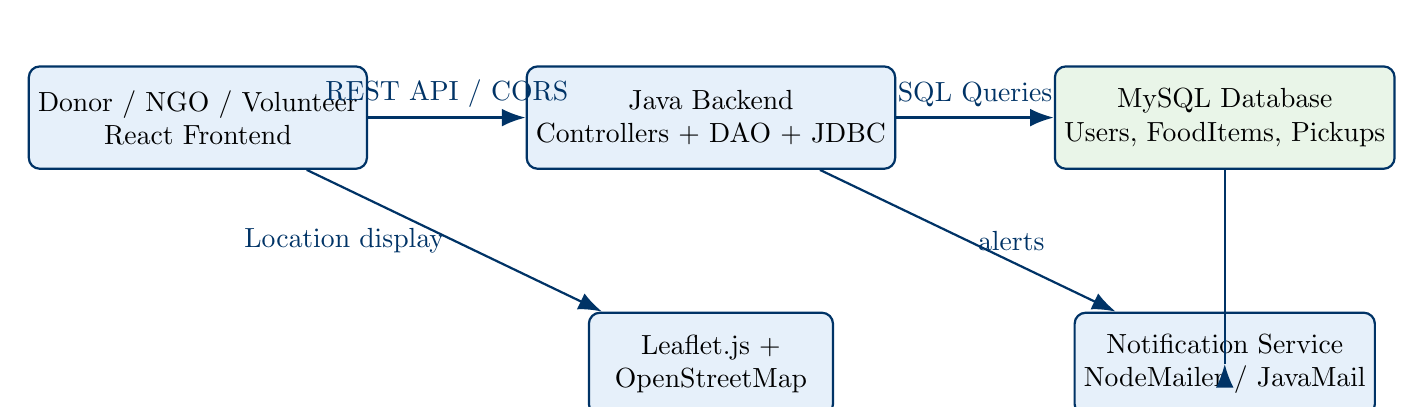
\begin{tikzpicture}[
box/.style={draw=darkblue, rounded corners, thick, fill=softblue, minimum width=3.1cm, minimum height=1.3cm, align=center},
dbox/.style={draw=darkblue, rounded corners, thick, fill=softgreen, minimum width=3.1cm, minimum height=1.3cm, align=center},
arrow/.style={-{Latex[length=3mm]}, thick, darkblue}
]
\node[box] (donor) {Donor / NGO / Volunteer\\React Frontend};
\node[box, right=2.0cm of donor] (backend) {Java Backend\\Controllers + DAO + JDBC};
\node[dbox, right=2.0cm of backend] (db) {MySQL Database\\Users, FoodItems, Pickups};
\node[box, below=1.8cm of backend] (map) {Leaflet.js +\\OpenStreetMap};
\node[box, below=1.8cm of db] (mail) {Notification Service\\NodeMailer / JavaMail};

\draw[arrow] (donor) -- node[above]{REST API / CORS} (backend);
\draw[arrow] (backend) -- node[above]{SQL Queries} (db);
\draw[arrow] (donor) -- node[left]{Location display} (map);
\draw[arrow] (backend) -- node[right]{alerts} (mail);
\draw[arrow] (db) |- (mail);
\end{tikzpicture}
\caption{High-Level Architecture of the \projecttitle{} System}
\end{figure}

\section{System Modules}
\begin{itemize}[leftmargin=1.2cm]
\item \textbf{Authentication Module:} Handles login and signup with role selection.
\item \textbf{Donation Module:} Allows donors to add food quantity, expiry time, and item status.
\item \textbf{NGO Dashboard Module:} Displays available food records for verification and claiming.
\item \textbf{Pickup Module:} Stores pickup assignments, latitude and longitude coordinates, and volunteer references.
\item \textbf{Map Module:} Displays donation and pickup locations through markers.
\item \textbf{Notification Module:} Sends alerts when food is added, claimed, or assigned.
\end{itemize}

\section{Database Design}
\begin{table}[H]
\centering
\caption{Database Schema Overview}
\renewcommand{\arraystretch}{1.4}
\begin{tabular}{@{} p{3cm} p{9.8cm} @{}}
\toprule
\textbf{Table} & \textbf{Important Attributes} \\
\midrule
Users & user\_id, name, email, password, role (Donor / Volunteer / NGO), phone \\
FoodItems & food\_id, food\_name, quantity, expiry\_time, status, donor\_id, created\_at \\
Pickups & pickup\_id, food\_id, volunteer\_id, ngo\_id, location\_lat, location\_long, pickup\_status \\
\bottomrule
\end{tabular}
\end{table}

\section{Entity Relationship Flow}
\begin{figure}[H]
\centering
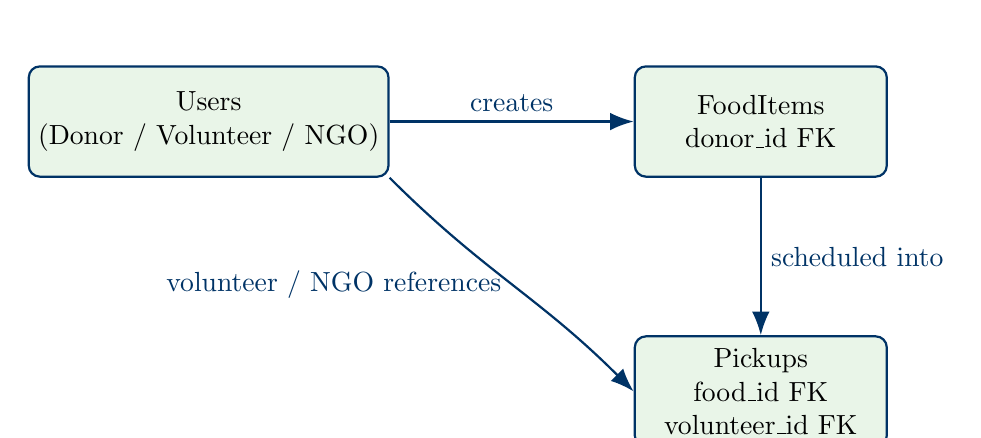
\begin{tikzpicture}[
ent/.style={draw=darkblue, rounded corners, thick, fill=softgreen, minimum width=3.2cm, minimum height=1.4cm, align=center},
arrow/.style={-{Latex[length=3mm]}, thick, darkblue}
]
\node[ent] (u) {Users\\(Donor / Volunteer / NGO)};
\node[ent, right=3.1cm of u] (f) {FoodItems\\donor\_id FK};
\node[ent, below=2.0cm of f] (p) {Pickups\\food\_id FK\\volunteer\_id FK};

\draw[arrow] (u) -- node[above]{creates} (f);
\draw[arrow] (f) -- node[right]{scheduled into} (p);
\draw[arrow] (u.south east) .. controls +(1.2,-1.2) and +(-1.2,1.2) .. node[left]{volunteer / NGO references} (p.west);
\end{tikzpicture}
\caption{Logical Entity Relationship Flow in \projecttitle}
\end{figure}

\section{API Design}
\begin{table}[H]
\centering
\caption{Core API Endpoints}
\renewcommand{\arraystretch}{1.35}
\begin{tabular}{@{} p{3cm} p{2cm} p{7.8cm} @{}}
\toprule
\textbf{Endpoint} & \textbf{Method} & \textbf{Purpose} \\
\midrule
/api/login & POST & Validates credentials and role-based access \\
/api/signup & POST & Registers a new donor, NGO, or volunteer \\
/api/add-food & POST & Stores food donation details in the database \\
/api/get-food & GET & Returns available food records for dashboard display \\
/api/pickups & POST / GET & Creates or retrieves pickup assignments \\
\bottomrule
\end{tabular}
\end{table}

\section{Application Workflow}
\begin{figure}[H]
\centering
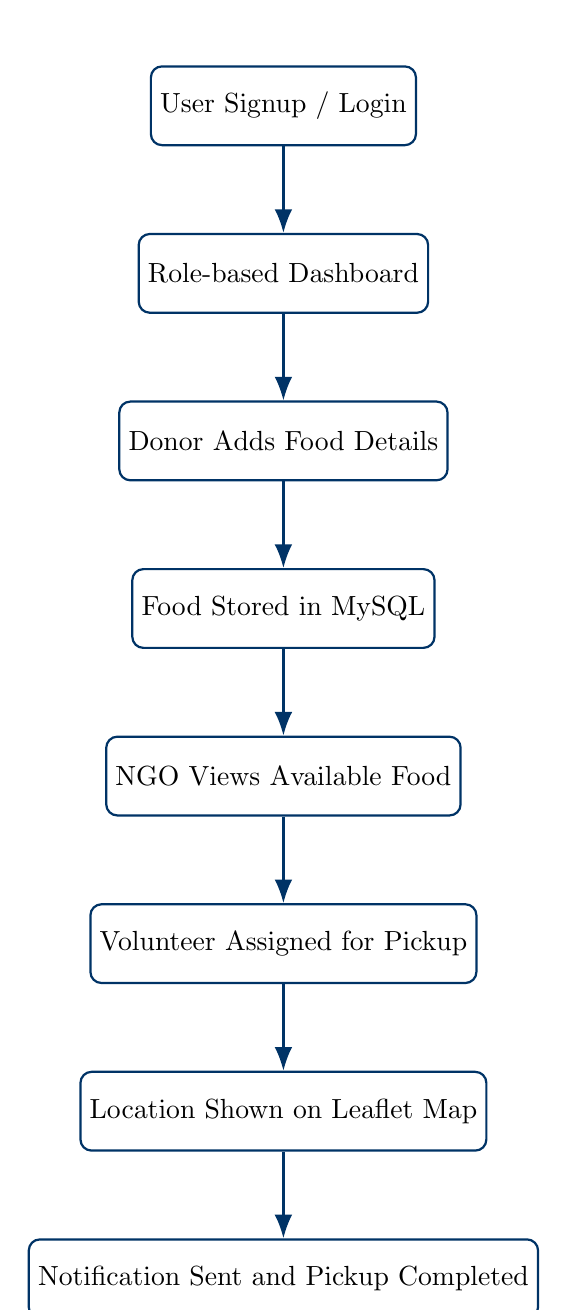
\begin{tikzpicture}[
flowstep/.style={draw=darkblue, rounded corners, thick, fill=white, minimum width=3.2cm, minimum height=1cm, align=center},
arrow/.style={-{Latex[length=3mm]}, thick, darkblue}
]
\node[flowstep] (s1) {User Signup / Login};
\node[flowstep, below=1.1cm of s1] (s2) {Role-based Dashboard};
\node[flowstep, below=1.1cm of s2] (s3) {Donor Adds Food Details};
\node[flowstep, below=1.1cm of s3] (s4) {Food Stored in MySQL};
\node[flowstep, below=1.1cm of s4] (s5) {NGO Views Available Food};
\node[flowstep, below=1.1cm of s5] (s6) {Volunteer Assigned for Pickup};
\node[flowstep, below=1.1cm of s6] (s7) {Location Shown on Leaflet Map};
\node[flowstep, below=1.1cm of s7] (s8) {Notification Sent and Pickup Completed};

\draw[arrow] (s1) -- (s2);
\draw[arrow] (s2) -- (s3);
\draw[arrow] (s3) -- (s4);
\draw[arrow] (s4) -- (s5);
\draw[arrow] (s5) -- (s6);
\draw[arrow] (s6) -- (s7);
\draw[arrow] (s7) -- (s8);
\end{tikzpicture}
\caption{Functional Workflow of the \projecttitle{} Application}
\end{figure}

\section{Frontend Design Considerations}
The frontend is designed using React.js with functional components and hooks. Key screens include login, signup, donor form, NGO dashboard, and map-based pickup view. The interface is intended to be clean, responsive, and impact-driven so that different user roles can use the application without confusion.

\section{Backend Design Considerations}
The backend follows a structured Java architecture with JDBC-based DAO classes. DAO separation improves maintainability and keeps database access logic independent from request handling. REST-style controllers or servlets process requests and return data to the frontend in a structured manner.

\chapter{Implementation Details}

\section{Frontend Implementation}
The React frontend includes:
\begin{itemize}[leftmargin=1.2cm]
\item Login and signup pages with role selection.
\item Donate Food form for donors such as hotels and hostels.
\item NGO dashboard displaying food item records in list form.
\item React-Leaflet integration for pickup location markers.
\item Responsive styling with a simple and impact-oriented visual hierarchy.
\end{itemize}

\section{Backend Implementation}
The Java backend includes:
\begin{itemize}[leftmargin=1.2cm]
\item Maven or Gradle project structure.
\item Database connection utility classes.
\item DAO classes for \texttt{Users}, \texttt{FoodItems}, and \texttt{Pickups}.
\item Controller or Servlet handling for \texttt{/api/login}, \texttt{/api/add-food}, and \texttt{/api/get-food}.
\item CORS support so the React application on port 3000 can communicate with the backend on port 8080.
\end{itemize}

\section{Database Initialization}
The database schema is designed for role-based access and food tracking. Foreign key relationships ensure integrity between donors, food items, and pickup assignments. SQL initialization scripts are part of the expected project deliverables for clean setup.

\section{Notification Handling}
To support pickup coordination, notifications can be implemented using either:
\begin{itemize}[leftmargin=1.2cm]
\item a lightweight Node.js microservice using NodeMailer, or
\item JavaMail API directly from the backend.
\end{itemize}
This flexibility allows the system to adapt based on hosting convenience and deployment strategy.

\section{Deployment Readiness and Documentation}
The project also requires supporting files such as \texttt{pom.xml}, \texttt{package.json}, and \texttt{README.md}. These files are important because they make the project reproducible, portable, and easier for evaluators or collaborators to set up.

\chapter{Internship Diary}

\renewcommand{\arraystretch}{1.5}
\footnotesize
\begin{longtable}{|p{1.8cm}|p{11.2cm}|}
\hline
\textbf{Week} & \textbf{Activities and Learning} \\
\hline
\endfirsthead
\hline
\textbf{Week} & \textbf{Activities and Learning} \\
\hline
\endhead
Week 1 & Understood the internship workflow, selected the social problem domain, and discussed the idea of a food redistribution platform. Learned how software requirements are derived from real-world community issues. \\
\hline
Week 2 & Studied the functional requirements of \projecttitle{} and identified the roles of donor, volunteer, and NGO. Prepared the initial feature list and workflow outline. \\
\hline
Week 3 & Designed the basic MySQL schema for users, food items, and pickups. Learned the importance of foreign keys, role-based data modeling, and normalized structure. \\
\hline
Week 4 & Planned the Java backend architecture with JDBC and DAO patterns. Understood separation between controllers, services, and data access logic. \\
\hline
Week 5 & Worked on authentication flow and role-based login logic. Improved understanding of request handling and response design in web applications. \\
\hline
Week 6 & Designed the Donate Food form and donor-side workflow. Learned how to capture quantity, expiry time, and food status meaningfully for real-world use. \\
\hline
Week 7 & Implemented NGO dashboard planning and food-list retrieval flow. Focused on clear data presentation and role-based dashboard behavior. \\
\hline
Week 8 & Explored React functional components and hooks for managing application state. Strengthened frontend structuring skills for reusable components. \\
\hline
Week 9 & Integrated map planning using Leaflet.js and OpenStreetMap. Learned how free mapping solutions can support location-aware applications effectively. \\
\hline
Week 10 & Designed the pickup assignment flow and volunteer coordination logic. Improved understanding of operational workflows within a full-stack system. \\
\hline
Week 11 & Studied notification integration using NodeMailer or JavaMail API. Learned how alerts can improve responsiveness in service-oriented applications. \\
\hline
Week 12 & Focused on CORS handling between React on port 3000 and Java backend on port 8080. Understood frontend-backend communication constraints. \\
\hline
Week 13 & Prepared system diagrams, API mapping, and module descriptions. Improved technical documentation and architectural presentation skills. \\
\hline
Week 14 & Reviewed implementation strategy, database setup instructions, and supporting configuration files such as README, package.json, and pom.xml. \\
\hline
Week 15 & Consolidated the complete report, refined technical explanations, and connected the project to sustainability and social impact outcomes. \\
\hline
\end{longtable}
\normalsize

\chapter{Technical Work}

\section{Project Title: \projecttitle}
\projecttitle{} is a full-stack food redistribution web application built to connect donors, NGOs, and volunteers. It is designed to reduce food waste and improve the speed and transparency of food sharing workflows.

\section{Core Features}
\begin{itemize}[leftmargin=1.2cm]
\item Role-based login and signup for Donor, Volunteer, and NGO.
\item Donation form with quantity, expiry time, and food status.
\item NGO dashboard for viewing available food items.
\item Pickup tracking with latitude and longitude coordinates.
\item Interactive map using React-Leaflet.
\item Notification support for food addition and pickup events.
\item REST communication between frontend and backend.
\end{itemize}

\section{Importance of the Chosen Architecture}
The architecture is suitable for learning and demonstration because each technology serves a clear purpose:
\begin{itemize}[leftmargin=1.2cm]
\item React.js provides modular, responsive frontend interaction.
\item Java and JDBC offer explicit backend logic and database connectivity.
\item MySQL ensures structured persistence of user and food data.
\item Leaflet.js enables free and practical map integration without paid APIs.
\item NodeMailer or JavaMail supports event-driven coordination.
\end{itemize}

\section{Expected Project Directory Structure}
\begin{figure}[H]
\centering
\fbox{
\parbox{0.9\textwidth}{
\ttfamily
FoodShare/\\
\hspace*{0.5cm}frontend/\\
\hspace*{1cm}src/\\
\hspace*{1.5cm}components/\\
\hspace*{1.5cm}pages/\\
\hspace*{1.5cm}services/\\
\hspace*{1cm}package.json\\
\hspace*{0.5cm}backend/\\
\hspace*{1cm}src/main/java/...\\
\hspace*{1cm}src/main/webapp/\\
\hspace*{1cm}pom.xml\\
\hspace*{0.5cm}database/\\
\hspace*{1cm}foodshare.sql\\
\hspace*{0.5cm}README.md
}
}
\caption{Expected Project Directory Structure for \projecttitle}
\end{figure}

\section{Advantages of the Project}
\begin{itemize}[leftmargin=1.2cm]
\item Reduces wastage of usable food.
\item Creates a structured communication channel among stakeholders.
\item Encourages community participation and volunteer engagement.
\item Uses accessible and mostly free technologies.
\item Can be extended into a real civic-tech or NGO-support application.
\end{itemize}

\section{Challenges and Considerations}
\begin{itemize}[leftmargin=1.2cm]
\item Accurate validation of food freshness and expiry data.
\item Handling role-based access cleanly across modules.
\item Reliable volunteer coordination and status updates.
\item Maintaining secure authentication and input validation.
\item Ensuring smooth API communication and deployment compatibility.
\end{itemize}

\section{Conclusion of Technical Work}
The \projecttitle{} project demonstrates how full-stack development can be applied to a meaningful social problem. It integrates frontend development, backend architecture, database design, location services, and notification workflows into one cohesive application model.

\chapter{Learning Outcomes}
\begin{itemize}[leftmargin=1.2cm]
\item Understood how to convert a social problem statement into a software solution.
\item Gained clarity in full-stack architecture involving React, Java, JDBC, and MySQL.
\item Learned the purpose and use of DAO patterns in backend application design.
\item Improved database design skills through role-based schema planning.
\item Learned how interactive maps can be used in logistics and service applications.
\item Strengthened documentation, workflow design, and requirement analysis skills.
\item Improved technical confidence in integrating multiple technologies into one project.
\item Understood how software projects can contribute to sustainability and social impact.
\end{itemize}

\chapter{Program Outcomes (POs) Addressed}

\begin{table}[H]
\centering
\caption{Program Outcomes Mapping}
\small
\renewcommand{\arraystretch}{1.5}
\begin{tabular}{@{} p{2cm} p{11cm} @{}}
\toprule
\textbf{PO Code} & \textbf{Contribution} \\
\midrule
\textbf{PO 1} & Applied engineering knowledge in web application planning, database design, backend logic, and role-based workflows. \\
\textbf{PO 2} & Identified the real-world problem of food wastage and analyzed how software can enable efficient redistribution. \\
\textbf{PO 3} & Designed a complete solution architecture for \projecttitle{} including frontend, backend, database, map, and notification modules. \\
\textbf{PO 5} & Used modern tools and technologies such as React.js, Java, JDBC, MySQL, Leaflet.js, and notification services. \\
\textbf{PO 9} & Improved communication and coordination skills by structuring the application around multi-stakeholder workflows. \\
\textbf{PO 11} & Developed independent learning and adaptability while exploring multiple technologies across the full-stack pipeline. \\
\bottomrule
\end{tabular}
\end{table}

\chapter{Student Reflection}
\begin{itemize}[leftmargin=1.2cm]
\item \textbf{Challenges:} One major challenge was structuring a complete full-stack system around a real-world problem while keeping the design practical and scalable. Understanding how frontend interaction, backend APIs, database integrity, maps, and notifications fit together required careful planning.

\item \textbf{Skills Gained:} The internship improved my confidence in system architecture, database design, role-based application workflows, React frontend planning, and Java backend thinking. It also strengthened my ability to prepare a technically organized report.

\item \textbf{Improvements Needed:} I would like to deepen my practical implementation skills in backend security, deployment, real email notification setup, and advanced state handling in frontend applications.
\end{itemize}

\chapter{Conclusion}
The internship at \companyname{} was a valuable academic and technical experience. Through the \projecttitle{} project, I was able to understand how software engineering concepts can be combined to solve a meaningful societal issue. The project brought together full-stack design, structured data handling, API planning, mapping, and workflow coordination in one coherent application idea.

More importantly, the internship helped me realize that software projects can create tangible community impact when designed with purpose. \projecttitle{} is a strong example of how technology can reduce waste, improve coordination, and support social good.

\chapter{References}
\begin{itemize}[leftmargin=1.2cm]
\item Vstand4U Solutions official website: \url{https://vstand4usolutions.com/}
\item React.js documentation: \url{https://react.dev/}
\item MySQL documentation: \url{https://dev.mysql.com/doc/}
\item Leaflet.js documentation: \url{https://leafletjs.com/}
\item OpenStreetMap project: \url{https://www.openstreetmap.org/}
\item Java JDBC documentation: \url{https://docs.oracle.com/javase/tutorial/jdbc/}
\item NodeMailer documentation: \url{https://nodemailer.com/}
\end{itemize}

\chapter{Annexure}

\section*{Attendance and Topic Summary}
\addcontentsline{toc}{section}{Attendance and Topic Summary}

\begin{table}[H]
\centering
\caption{15-Week Attendance Report}
\renewcommand{\arraystretch}{1.4}
\begin{tabular}{|c|p{9cm}|c|}
\hline
\textbf{Timeline} & \textbf{Topic} & \textbf{Remark} \\
\hline
Week 1 & Internship orientation and problem selection & Present \\
\hline
Weeks 2--3 & Requirement analysis and database schema planning & Present \\
\hline
Weeks 4--5 & Java backend architecture and authentication flow & Present \\
\hline
Weeks 6--8 & React frontend planning and dashboard design & Present \\
\hline
Weeks 9--10 & Leaflet map integration and pickup workflow & Present \\
\hline
Weeks 11--12 & Notification handling and CORS coordination & Present \\
\hline
Weeks 13--15 & Documentation, diagrams, and final report preparation & Present \\
\hline
\end{tabular}
\end{table}

\section*{Recommended Deliverables for the Actual Project Repository}
\addcontentsline{toc}{section}{Recommended Deliverables for the Actual Project Repository}
\begin{itemize}[leftmargin=1.2cm]
\item \texttt{README.md} with setup instructions.
\item SQL file for database initialization.
\item \texttt{pom.xml} for Java backend configuration.
\item \texttt{package.json} for React frontend dependencies.
\item Source directories for frontend, backend, and database scripts.
\item CORS configuration and environment notes for local execution.
\end{itemize}

\end{document}
